
\begin{Exercise}[label={footfall_analysis}]
A concrete ribbed slab floor spans 9 m and has an average mass of \SI{500}{kg/m^2}. The floor is simply supported on either side and has a natural frequency of vibration of \SI{6.3}{Hz}. 
The floor is to be used for aerobics and other similar rhythmic activities at frequencies ranging from 1.5 to \SI{2.5}{Hz} and with contact ratios $\alpha$ between 0.5 and 1. During these activities the average imposed load will remain below \SI{0.75}{kN/m^2} (before dynamic magnification) and the damping ratio can be taken to be \SI{3}{\%}.

\begin{enumerate}[(a)]
    \item Determine the maximum possible resonant displacement and the resulting peak acceleration and bending moment per unit width.
    \item If the floor has been designed for a service load of \SI{5}{kN/m^2}, determine its suitability for the proposed use.
\end{enumerate}

\begin{center}
\pictures{beamPeople}
\hspace{1em}
\pictures{contactRatio}
\end{center}

\shortAnswer (a) $u_\text{max} = \SI{7}{mm}$, $M_\text{max} = \SI{250}{kN.m/m}$, $a_\text{max} = \SI{9}{m/s^2}$. (b) The floor is not suitable for aerobics.\\
References: \cite{chopra}
\end{Exercise}



\begin{Answer}[ref={footfall_analysis}]
The structure properties per unit width using a sine shape function are
$$
m = \int_{0}^{l}w\psi^2dx = \int_{0}^{l}w\sin^2\left(\frac{\pi x}{l}\right)dx = \frac{wl}{2} = \frac{500\times9}{2} = \SI{2250}{kg/m},
$$
$$
k = \omega^2m = \left(2\pi6.3\right)^2\times2250 = \SI{3500}{kN/m^2},
$$
and the equivalent force for the shape function $\psi$ is
$$
\hat{F} = \int_{0}^{l}F\psi dx = \frac{2Fl}{\pi} = \SI{4.3}{kN/m}.
$$
The transient walking force considered is a periodic loading with a piecewise definition. Because the action is periodic, a different approach from that of Example \ref{moving_load} can be followed. The action will be approximated using a Fourier series, which is suitable for any periodic action.

\paragraph{Pre-computed Fourier terms}

Each component of a Fourier series is also known as a harmonic. For a half sine activity, the amplitudes of the first four harmonics are the following:

\begin{center}
\begin{tabular}{|l|c|cccc|}
    \hline
    Activity & $\alpha$ & $F_1/F_{avg}$ & $F_2/F_{avg}$ & $F_3/F_{avg}$ & $F_4/F_{avg}$ \\ \hline
    Walking  &    2/3   &   1.29   &   0.16   &   0.13   &   0.04   \\
    Exercise &    1/2   &   1.57   &   0.67   &   0.00   &   0.13   \\
    Jumping  &    1/3   &   1.80   &   1.29   &   0.67   &   0.16   \\
    High jumping & 1/4  &   1.89   &   1.57   &   1.13   &   0.67   \\ \hline
\end{tabular}
\end{center}
Then, the dynamic force is the superposition of the static force and the harmonics multiplied by the corresponding dynamic magnification factor:
$$
F_\text{dyn} = F_\text{avg} + H_1F_1 + H_2F_2 + H_3F_3 + \dots
$$
At this point is is crucial that finding the maximum excitation is not a direct problem, since it depends on two free parameters, the walking frequency and the contact ratio depending on the type of activity. Instead of performing a trial error evaluation of each possible combination of frequencies and contact ratios, we will select them carefully by inspecting the table of predefined Fourier terms. It is reasonable to assume that the maximum response will happen when some of the harmonics are in ressonance. Thus, we choose a base frequency of $2.1$ for the contact ratio $2/3$, and a base frequency of $1.58$ for the contact ratio equal to $0.5$.

When $\alpha=2/3$ and the frequency $f_1=\SI{2.1}{Hz}$, the third mode will be in ressonance. Then, we have the following magnification factors,
\begin{align*}
\gamma_1 = \frac{2.1}{6.3} = 0.33\ &\rightarrow\ H_1 = \frac{1}{\sqrt{(1-0.33^2)^2 + 4\times0.03^2\times0.33^2}} = 1.12\\
\gamma_2 = \frac{4.2}{6.3} = 0.66\ &\rightarrow\ H_1 = \frac{1}{\sqrt{(1-0.66^2)^2 + 4\times0.03^2\times0.66^2}} = 1.8\\
\gamma_3 = \frac{6.3}{6.3} = 1.0\ \ &\rightarrow\ H_1 = \frac{1}{\sqrt{(1-1.0^2)^2  + 4\times0.03^2\times1.0^2}}  = 16.7\\
\gamma_4 = \frac{8.4}{6.3} = 1.33\ &\rightarrow\ H_1 = \frac{1}{\sqrt{(1-1.33^2)^2 + 4\times0.03^2\times1.33^2}} = 1.28\ .
\end{align*}

When intersted in computing the maximum displacement corresponding to the moving load, the average deflection shall be taken into account in addition to the harmonic components,
$$
u_\text{max} = \frac{\hat{F}_\text{avg}}{k} (1 + 1.12\cdot1.29 + 1.8\cdot0.16 + 16.7\cdot0.13 + 1.28\cdot0.04) = 5.0\frac{\hat{F}_\text{avg}}{k}.
$$

Similarly, when the type of activity is classified as exercise, the contact ratio $\alpha$ is $0.5$ and we will consider ressonance at the fourth harmonic, i.e., $f_1=\SI{1.58}{Hz}$. The maximum displacement according to it will be
$$
u_\text{max} = \frac{\hat{F}_\text{avg}}{k} (1 + 1.07\cdot1.57 + 1.34\cdot0.67 + 0.0 + 16.7\cdot0.13) = 5.7\frac{\hat{F}_\text{avg}}{k}.
$$

After this analysis, it is possible to conclude that the maximum response will happen when the contact ratio $\alpha=0.5$ and the frequency $f_1=\SI{1.58}{Hz}$. The corresponding displacement and bending moment per unit width will be found as

$$
u_\text{max} = 5.7\frac{\hat{F}_\text{avg}}{k} = 5.7\frac{4.3}{3500} = \SI{7e-3}{m} = \SI{7}{mm},
$$
$$
M_\text{max} = 5.7\frac{\hat{F}_\text{avg}\, l^2}{8} = 5.7\frac{0.75\times9^2}{8} \approx \SI{250}{kN.m/m}.
$$

On top of the previously calculated values, accelerations are a very common measure for human confort. When interested in maximum accelerations, only the contribution from the harmonics will be considered, because the time derivative of the average value is zero by definition. The acceleration

$$
a_\text{max} = 4.7\frac{\hat{F}_\text{avg}}{m} = 4.7\frac{4.3}{2.25} = \SI{9}{m/s^2},
$$

is extremely high due to the lisghtweight floor. While the ribbed floor is suitable for this activity from the point of view of displacements and bending moments, the acceleration is -by far- over the threshold of \SI{0.5}{\%} of the gravity. Thus, the floor slab is not suited for this activity.


\paragraph{Calculation of the Fourier terms}
Most commonly, Fourier series are expressed as a linear combination of $\sin$ and $\cos$,
$$
F(t) \approx \frac{a_0}{2} + \sum_{n=0}^{\infty} \left(a_n\cos(n\Omega t) + b_n\sin(n\Omega t)\right)\, ,
$$
with coefficients
\begin{align*}
a_0 &= \frac{2}{T}\int_{0}^{T} F(t) dt \, , \\
a_n &= \frac{2}{T}\int_{0}^{T} F(t) \cos(n\Omega t) dt \, , \\
b_n &= \frac{2}{T}\int_{0}^{T} F(t) \sin(n\Omega t) dt \, .
\end{align*}

An alternative representation consists in combining the trigonometric functions as
$$
F(t) \approx F_0 + \sum_{n=0}^{\infty} F_n\sin(n\Omega t + \phi_n) \, ,
$$
with the new coefficients
\begin{align*}
&F_0 = \frac{a_0}{2} \, , \\
&F_n = \sqrt{a_n^2 + b_n^2} \, , \\
&\tan\phi_n = \frac{b_n}{a_n} \, . \\
\end{align*}


\begin{center}
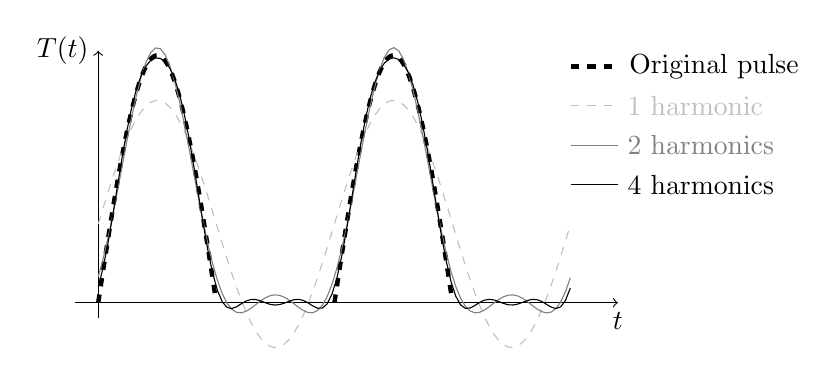
\begin{tikzpicture}[domain=0:2, xscale=3, samples=100]
    \draw[->] (-0.1,0) -- (2.2,0) node[below] {$t$};
    \draw[->] (0,-0.2) -- (0,3.2) node[left] {$T(t)$};

    % '\x r' means to convert '\x' from degrees to radians:
    \draw[ultra thick,dashed,domain=0:0.5] plot (\x,{pi*sin(2*pi*\x r)});
    \draw[ultra thick,dashed,domain=1:1.5] plot (\x,{pi*sin(2*pi*\x r)});
    \draw[lightgray,dashed] plot (\x,{1+1.57*sin(2*pi*\x r)});
    \draw[gray] plot (\x,{1+1.57*sin(2*pi*\x r)-0.67*cos(4*pi*\x r)});
    \draw[black] plot (\x,{1+1.57*sin(2*pi*\x r)-0.67*cos(4*pi*\x r)-0.13*cos(8*pi*\x r)});

    \draw[ultra thick,dashed] (2,3)   -- +(.2,0) node[right] {Original pulse};
    \draw[lightgray,dashed]   (2,2.5) -- +(.2,0) node[right] {1 harmonic};
    \draw[gray]               (2,2)   -- +(.2,0) node[right] {2 harmonics};
    \draw[black]              (2,1.5) -- +(.2,0) node[right] {4 harmonics};
\end{tikzpicture}
\end{center}

\end{Answer}
